
  
  This section includes the analysis and evaluation of the realistic case, that is, the case where both reading and writing requests are possible, with their respective probabilities of occurrence listed in table \ref{tab:type_requests}. In addition, we considered the waiting between requests, load distribution and connection pool, as we just mentioned in the last section.

  We believe it would be best to do an analysis of how each request influenced the big picture, before evaluating metrics regarding throughput and response time. As such, we present Table \ref{tab:geral_real} on the next page.
  
\begin{sidewaystable}[h!]
    \centering
    \begin{tabular}{|l|l|l|l|l|l|}
      \hline
      \textbf{Request} & \textbf{\# Requests} & \textbf{\# Fails} & \textbf{Average (ms)} & \textbf{Average size (bytes)} & \textbf{RPS} \\ 
      \hline
      GET /current\_package\_list\_with\_resources & 756 & 55 & 17890 & 369734 & 3.0    \\ 
      \hline
      GET /resource\_show?id & 626 & 38 & 16830 & 763 & 2.5   \\ 
      \hline
      GET /package\_show?id & 799 & 32 & 14279 & 10652 & 3.2    \\
      \hline
      GET /organization\_list & 481 & 25 & 15864 & 124 & 1.9   \\
      \hline
      GET /group\_list & 473 & 19 & 13284 & 113 & 1.9   \\
      \hline
      POST /package\_create & 163 & 118 & 18232 & 1063 & 0.7   \\ 
      \hline
      POST /package\_revise & 138 & 16 & 23257 & 4577 & 0.6   \\ 
      \hline
      POST /resource\_create\_default\_resource\_views & 109 & 5 & 12272 & 332 & 0.4   \\ 
      \hline
      POST /datastore\_create & 101 & 5 & 15491 & 106 & 0.4    \\
      \hline
      Aggregated & 3646 & 313 & 16166 & 79395 & 14.5   \\ 
      \hline
    \end{tabular}
    \caption{\label{tab:geral_real}Request statistics for reading and writing requests}
\end{sidewaystable}
    \clearpage% Flush page

  
  As we can already see, the two biggest times are the two for writing requests, and so we already have an idea of how influential these are going to be in the big picture. Also, the number of total requests, as we can see, is the lowest so far, which was also to be expected.
    
  \subsection{Throughput}
  
  For this metric, we already know that adding write requests will have impact on the number of requests executed per second.
  
  \begin{figure}[H]
    \centering
    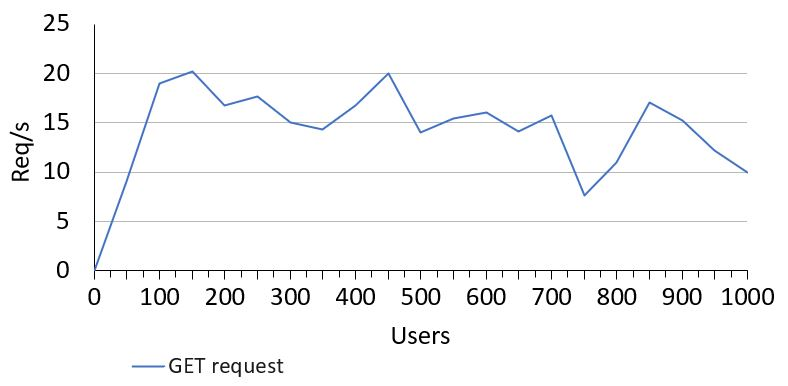
\includegraphics[width=.8\textwidth]{img/performance_evaluation/real.JPG}
    \caption{\label{tab:throughput_real}Throughput for reading and writing requests}
  \end{figure}
  
  We can then conclude from the Figure \ref{tab:throughput_real} the following: 
  
  \begin{itemize}
      \item There is a certain balance in the values from start to finish, which highlights the factors considered (without them, we would certainly have to reduce the sample of users);
      \item The 100-user mark proves to be the optimal number of concurrency, since in addition to reaching the maximum peak of 19 requests per second, we consider that a user would make 1 request every 4 seconds, which making the proportion, 100 users would make a total of 25 req/s, which being a bit higher than the 19 req/s would have a slight affect at the level of response time.
  \end{itemize}. 
  
  
  \subsection{Response time}
  
  For response time, we also expect the worst result so far. Nevertheless, we expect that the median response time variation, like throughput, will not show a considerable range between users.
  
  \begin{figure}[H]
    \centering
    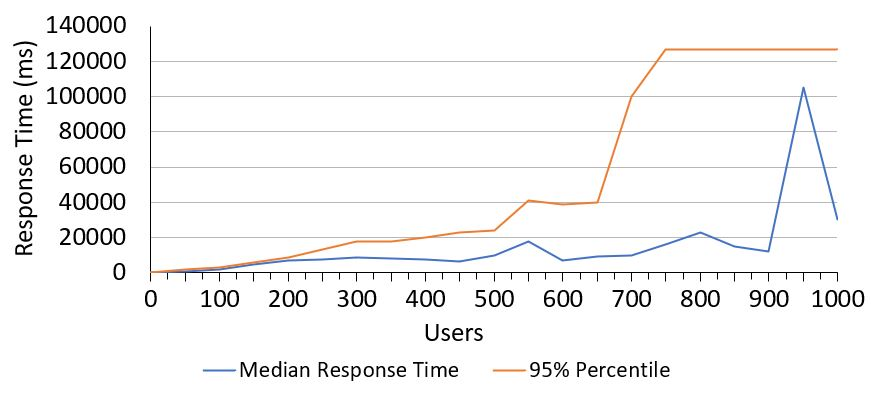
\includegraphics[width=1\textwidth]{img/performance_evaluation/real_time.JPG}
    \caption{\label{tab:time_real}Response time for reading and writing requests}
  \end{figure}
  
  Figure \ref{tab:time_real} tells us that:
  
  \begin{itemize}
      \item In fact, the variation of the median is not as considerable as in most of the cases already worked on, although its sharpest rise starts earlier, from the 50 users, which registers a 420 ms mark as far as the median is concerned, while the 100 users that we had referenced as the competition ideal, registers 1900 ms;
      \item The 95\% percentile ends up showing a balanced growth without peaks until it reaches a maximum peak of 127000 ms at 750 users and then stabilises.
  \end{itemize}
  
\newpage  
  
  \subsubsection{CPU and Disk Utilisation}
  
  In a realistic scenario, we believe that the CPU utilisation will be the same as obtained from the scenarios with load distribution and that the Disk utilisation will show a marked difference from what we have analysed so far, due to the write requests. To scrutinise what we have stated, we present the Table \ref{tab:cpu_real}.

\begin{table}[h!]
\centering
\begin{tabular}{|c|c|c|c|c|} 
\hline
\multirow{2}{*}{\textbf{Users }} & \multirow{2}{*}{\textbf{~\%CPU}} & \multicolumn{3}{c|}{\textbf{Devices}}                     \\ 
\cline{3-5}
                                 &                                  & \textbf{tps} & \textbf{kB\_read/s} & \textbf{kB\_wrtn/s}  \\ 
\hline
100  & 10,0 & 111,8  & 0,2  &  3814,8                   \\ 
\hline
500  & 10,1 & 151,7 & 0,5 & 8023,8                    \\ 
\hline
1000 & 9,5 & 90,5 & 0,4 & 4743,1                 \\ 
\hline
\end{tabular}\caption{\label{tab:cpu_real}CPU and Disk utilisation}
\end{table}

Thus, we conclude that what we predicted actually happens. The number of kB written per second increases considerably due to the existence of write requests on the devices, which consequently causes differences in the total data present in the system, and so when read requests are made, it is necessary to access the disk to access the new data, which are not yet in RAM and then in the CPU cache.

  
  \subsection{Summary}
  
  We conclude this section with a positive balance. Based on what we have just examined, we can consider that the ideal number of users of our system would be 100 users and would serve for research teams from an institute like \gls{inesctec} to work on the platform. However, recognizing the pessimistic estimate we have, we are confident that in a real world scenario our system could possibly handle far more users, as well as enjoying an improvement of the available resources.
  